\documentclass[a4paper]{article}
\usepackage[utf8]{inputenc}
\usepackage[english]{babel}
\usepackage{hyperref}
\usepackage{url}
\usepackage{enumerate}
\usepackage{subfiles}
\usepackage[lmargin=3cm,rmargin=3cm,tmargin=2.5cm,bmargin=2.5cm]{geometry}
\usepackage{titlesec}
\usepackage{todonotes}
\usepackage{graphicx}
\usepackage{parskip}
\usepackage[newfloat]{minted}
\usepackage{lastpage}
\usepackage{fancyhdr}
\usepackage[titletoc,toc,title]{appendix}

\definecolor{linkcol}	{RGB}	{42, 93, 176}
\definecolor{monokaibg} {RGB} 	{41, 42, 35}

\setminted{linenos=false, breaklines, breakanywhere, numbersep=5pt, framesep=2pt, autogobble, xleftmargin=10pt, xrightmargin=27pt, fontsize=\footnotesize, bgcolor=monokaibg}
\usemintedstyle{monokai}
\SetupFloatingEnvironment{listing}{name=Code Snippet}
\SetupFloatingEnvironment{listing}{listname=List of Code Snippets}

%Package setup
\hypersetup{
colorlinks=true,
linktoc=all,
linkcolor=black,
citecolor=magenta,
urlcolor=linkcol,
}


\title{HazzardHulen.io\\[4cm]
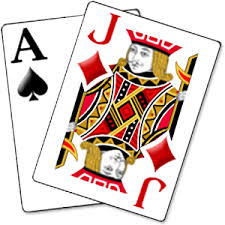
\includegraphics[width=.7\textwidth]{../blackjack}
\vfill}
\author{
  Thomas A. Lemqvist\\
  \texttt{thlem14@student.sdu.dk}
}

\begin{document}
\pagestyle{fancy}
\fancyhf{}
\rhead{Thomas A. Lemqvist}
\lhead{
\includegraphics[height=1cm]{images/sdu-header.png} HazardHulen.IO}

\maketitle
\thispagestyle{empty}
\newpage
\hspace{0cm}
\vfill
\tableofcontents

\vfill

\section*{Acknowledgements}
This paper exceeds the five page limit, due to the usage of images and code snippets, If they were removed, it will abide the limit.

\vfill
\newpage

\rfoot{Page \thepage\ of \pageref{page_b4_appendices}}
\setcounter{page}{1}


% #=#=#=#=#=#=#=#=#=#=#=#=#=#=#=#=#=#=#=#=#=#=#=#=#=#=#=#=#=#=#=#=#=#=#=#=#=#=#=#=# 


\section{Introduction}
\textit{This section introduces the application developed in the TEC course.}

Together with a group of classmates, I created a Black Jack web-application, nicknamed HazardHulen.io, where users can "sit" at the table and bet game money.

\begin{figure}[H]
  \centering
  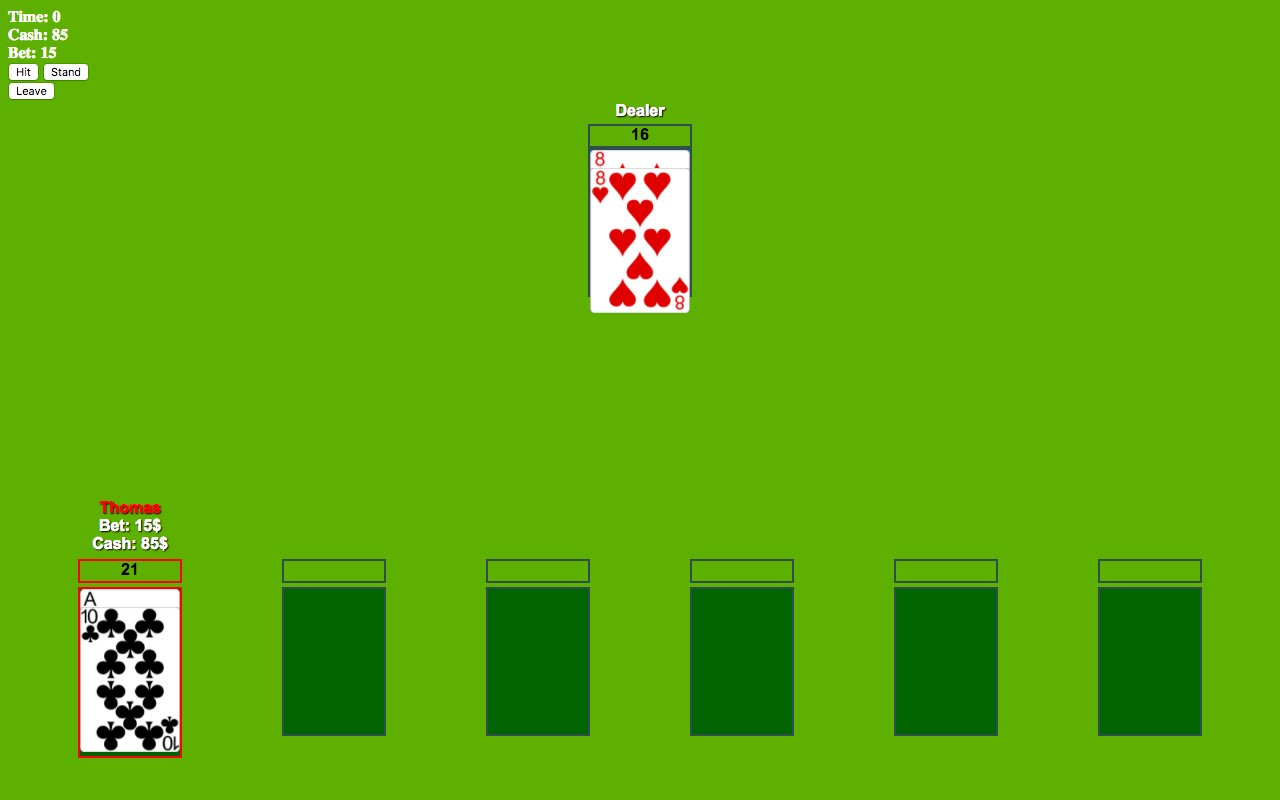
\includegraphics[width=0.5\textwidth]{images/singleplayer}	
  \caption{Singleplayer in the Black Jack web-App}
  \label{sp:bj}
\end{figure}

\autoref{sp:bj} shows the black jack table with one player, and the dealer AI, who makes decisions based on the score of his cards, to follow some common black jack dealer rules.

The game also scales to multiple players, currently only up to 6 players, due to the lack of table space. This could be changed, by introducing multiple tables to the system.

\begin{figure}[hbt]
  \centering
  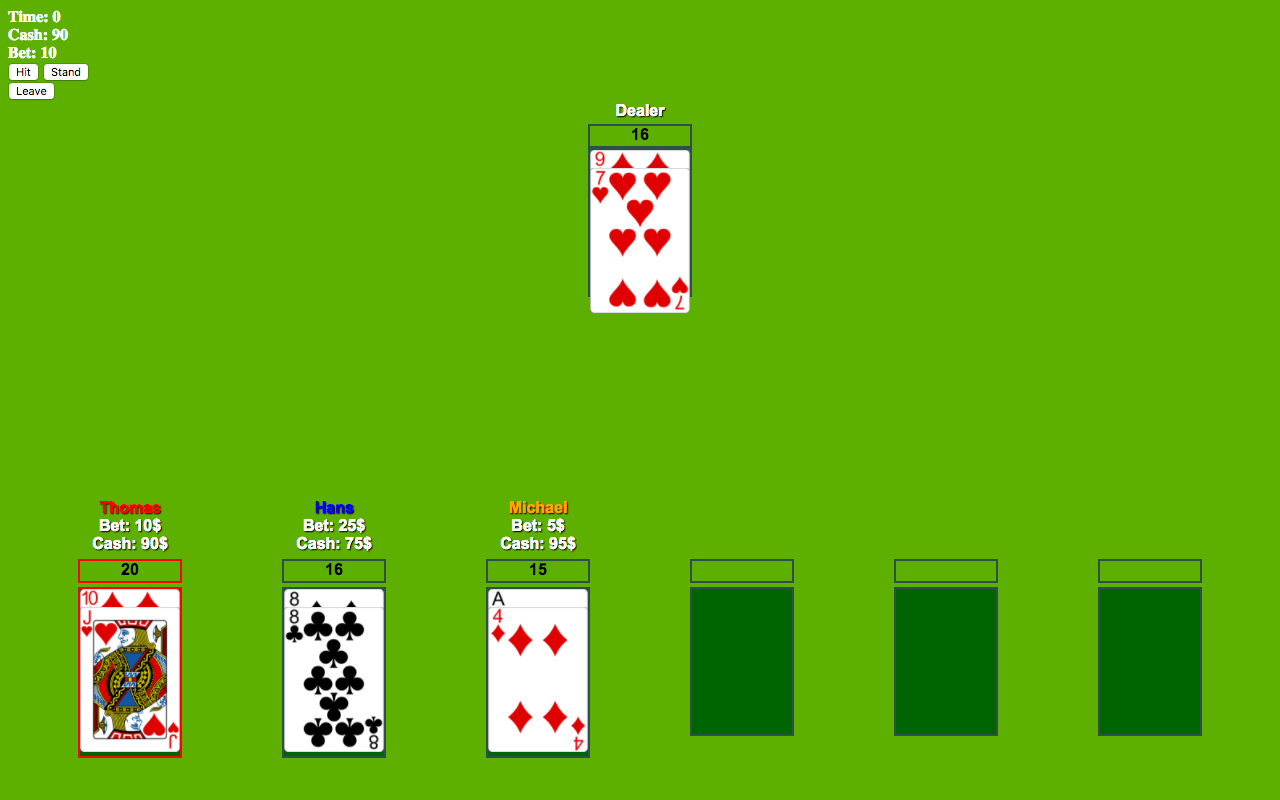
\includegraphics[width=0.5\textwidth]{images/multiplayer}	
  \caption{Multiplayer in the Black Jack web-App}
  \label{mp:bj}
\end{figure}

\autoref{mp:bj} shows three players sitting at the table. The player whose currently taking his turn is highlighted with a red edge around his score and cards.

Instructions upon how this can be run can be found in appendix \autoref{app_h2r}


% #=#=#=#=#=#=#=#=#=#=#=#=#=#=#=#=#=#=#=#=#=#=#=#=#=#=#=#=#=#=#=#=#=#=#=#=#=#=#=#=#


\section{Technologies}
\label{sec_tech}
\textit{This section introduces technologies, which was chosen to work with.}
\subsection{TypeScript}
TypeScript is a superset of JavaScript, and adds a more Object Oriented (OO) abstraction to JavaScript. It does this, by allowing the developer to write in a OO style, with interfaces, classes etc.\\
One of TypeScripts core features, is the ability to specify types for variables (number, string, and boolean). This makes it easier for developers to avoid errors, where strings are inserted into numbers.\\
The TypeScript file can be compiled into plain JavaScript, which can then be deployed \cite{tsc}.

It can be implemented to easily configure the object structure of the system, in the case of HazardHulen.IO, it can be used to model the Table and Player objects.

\begin{figure}[hbt]
  \centering
  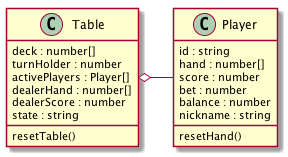
\includegraphics[width=0.6\textwidth]{../UpdatedClassDiag}
  \caption{Class Diagram for HazardHulen.IO}
  \label{img_class_diag}
\end{figure}

\subsection{Cros Site Scripting Protection}
Cross Site Scripting (xss) is the injection of client side scripts into other clients, this can be done in comments or names, really anything which shows on other clients as embedded text.\\
it works by entering a \texttt{<script>...</script>} tag into a comment, this will be read by other clients as part of the websites own scripts and executed \cite{xss}.

It can easily be prevented, simply by escaping the significant xss characters, in any input fields which shows text to other clients \cite{xss-prep}.


% #=#=#=#=#=#=#=#=#=#=#=#=#=#=#=#=#=#=#=#=#=#=#=#=#=#=#=#=#=#=#=#=#=#=#=#=#=#=#=#=#


\section{Implementation}
\label{sec_imp}
\textit{This section describes the implementation of the technologies mentioned in \autoref{sec_tech}}
\subsection{Implementation og TypeScript}
Because TypeScript (ts) is a superset of JavaScript (js), it is actually really easy to transfer the functionality from js to ts.

I have reimplemented the server in TypeScript.

I started by changing the file extension from \textit{app.js} to \textit{app.ts}, which is the TypeScript extension.

I then opened the a command line, and entered the \textbf{\texttt{\$ tsc -w app.ts}} command, which compiles the app.ts file, each time it is changed. (-w = watchmode, which compiles on save)

\begin{listing}[H]
\begin{minted}[firstnumber=1]{typescript}
class Table {
    deck : number[];
    turnHolder : number;
    activePlayers : Player[];
    dealerHand : number[];
    dealerScore : number;
    state : string;

    constructor(){
        this.activePlayers = [];
        this.resetTable();
    }

    public resetTable() {
        this.deck = _.shuffle(_.range(1, 52));
        this.dealerHand = [];
        this.dealerScore = 0;
        this.state = 'idle';
        this.turnHolder = 0;
    }
    
}
\end{minted}
\caption{TypeScript implementation of the table Object}
\label{lst_table}
\end{listing}

I then implemented the table object, shown in \autoref{lst_table}. It has specified types on its variables.

\begin{listing}[H]
\begin{minted}[firstnumber=1]{javascript}
var Table = (function () {
    function Table() {
        this.activePlayers = [];
        this.resetHands();
    }
    Table.prototype.resetHands = function () {
        this.deck = _.shuffle(_.range(1, 52));
        this.dealerHand = [];
        this.dealerScore = 0;
        this.state = 'idle';
        this.turnHolder = 0;
    };
    return Table;
}());
\end{minted}
\caption{the compiled Table}
\label{lst_table_compiled}
\end{listing}


\autoref{lst_table_compiled} shows the js code, which was generated form the ts code in \autoref{lst_table}. It is plain JavaScript, and can be executed to have the server running.


\subsection{Implementation of Cross Site Scripting Protection}
I started by identifying the places in the front end, which could be vulnerable to injection attacks.

And i found two places. when the player has to set his nickname, and when he has to bet, it is possible to inject code into these input fields.

I figured that i could just make a function which escaped the significant characters \cite{xss-prep}.

\begin{listing}[H]
\begin{minted}[]{javascript}
        function validateInputForJs(input) {
            input = input.replace(/(&)/g,   "&amp");
            input = input.replace(/(<)/g,   "&lt");
            input = input.replace(/(>)/g,   "&gt");
            input = input.replace(/(")/g,   "&quot");
            input = input.replace(/(')/g,   "&#x27");
            input = input.replace(/(\/)/g,  "&#x2F");
            return input;
        }
\end{minted}
\caption{Function which escapes significant XSS characters.}
\label{lst_xss_escape}
\end{listing}

\autoref{lst_xss_escape} shows the function which escapes the significant characters:[ \texttt{\&, $<$, $>$, ", ', /}], by locating them in the string by using regex \cite{regex}, and then replacing them with their hex representation. This will make them be appear as if they didn't change, but they will not be executed as scripts anymore.


% #=#=#=#=#=#=#=#=#=#=#=#=#=#=#=#=#=#=#=#=#=#=#=#=#=#=#=#=#=#=#=#=#=#=#=#=#=#=#=#=#


\section{Comparison}
\textit{This section analyses and discusses the impact of the implementation in \autoref{sec_imp}}


\subsection{TypeScript}

I decided to test the responsiveness of the "new" server, to see if the TypeScript implementation had had an impact on this.

I found a tool called loadtest \cite{loadtest}, which can be used to test the responsiveness of a Node server. It does this by setting up concurrent sessions, which makes requests to the specified target, it is very similar to a "controlled" dos attack\footnote{denial of service attack \url{https://en.wikipedia.org/wiki/Denial-of-service_attack}}.

\begin{listing}[H]
\centering
\begin{minted}[firstnumber=1, bgcolor=white]{sh}
$ loadtest -t 60 -c 20 --rps 300 http://localhost:13337
\end{minted}
\caption{The command to execute the loadtest.}
\label{lst_loadtest}
\texttt{-t = time   -c = number of sessions  --rps = requests/second}
\end{listing}

\autoref{lst_loadtest} shows the command I used to test the server responsiveness. I tested for 60 seconds, with 20 concurrent sessions, and 300 requests per second.\\

The tool then returns information about the responsiveness of the server, and gives a mean latency.




\subsection{Cros Site Scripting}
I tested this, on an older version of the application, by setting my nickname as \texttt{<script>alert('Andy says hello')</script>Andy}

\begin{center}
	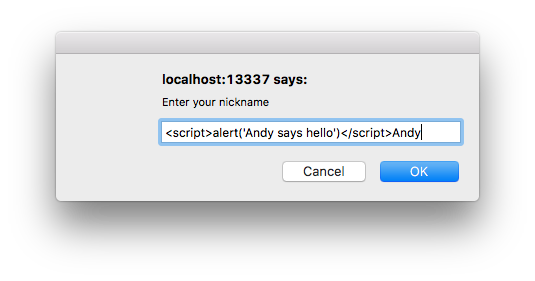
\includegraphics[width=.5\textwidth]{images/xss_input}
\end{center}

This resulted in my nick name becomming Andy (see \autoref{img_xss_succes}), and a alert message popping up each time someone does anything. This is really annoying, but it is far from the worst thing one could do with xss, this example is very loud (and visual), it could potentially be used to download malware unto an unsuspecting user machine \cite{xss_consequences}.

\begin{figure}[H]
  \centering
  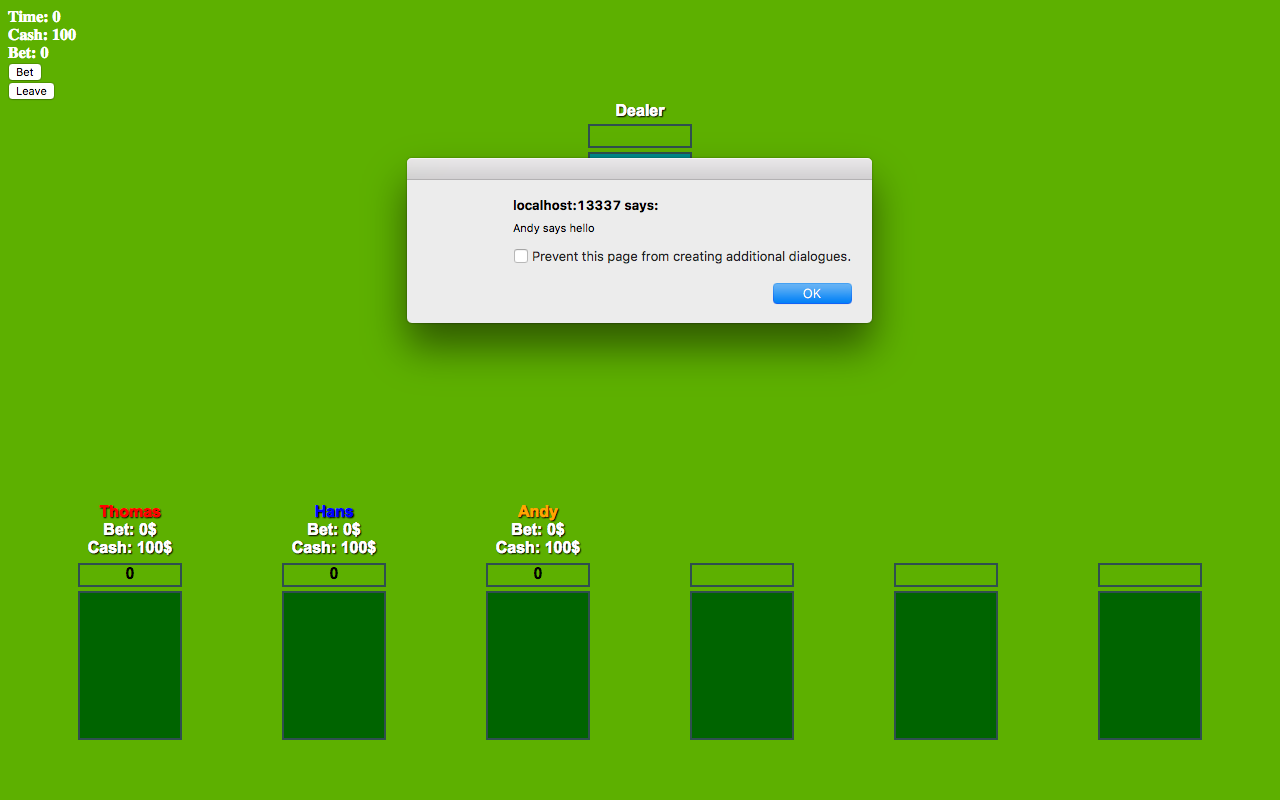
\includegraphics[width=0.65\textwidth]{images/xss_dialog}
  \caption{Image showing the dialog, as a result of the xss injection}
  \label{img_xss_succes}
\end{figure}


I then did the exact same thing, on the version which implements the escape function.

\begin{figure}[H]
  \centering
  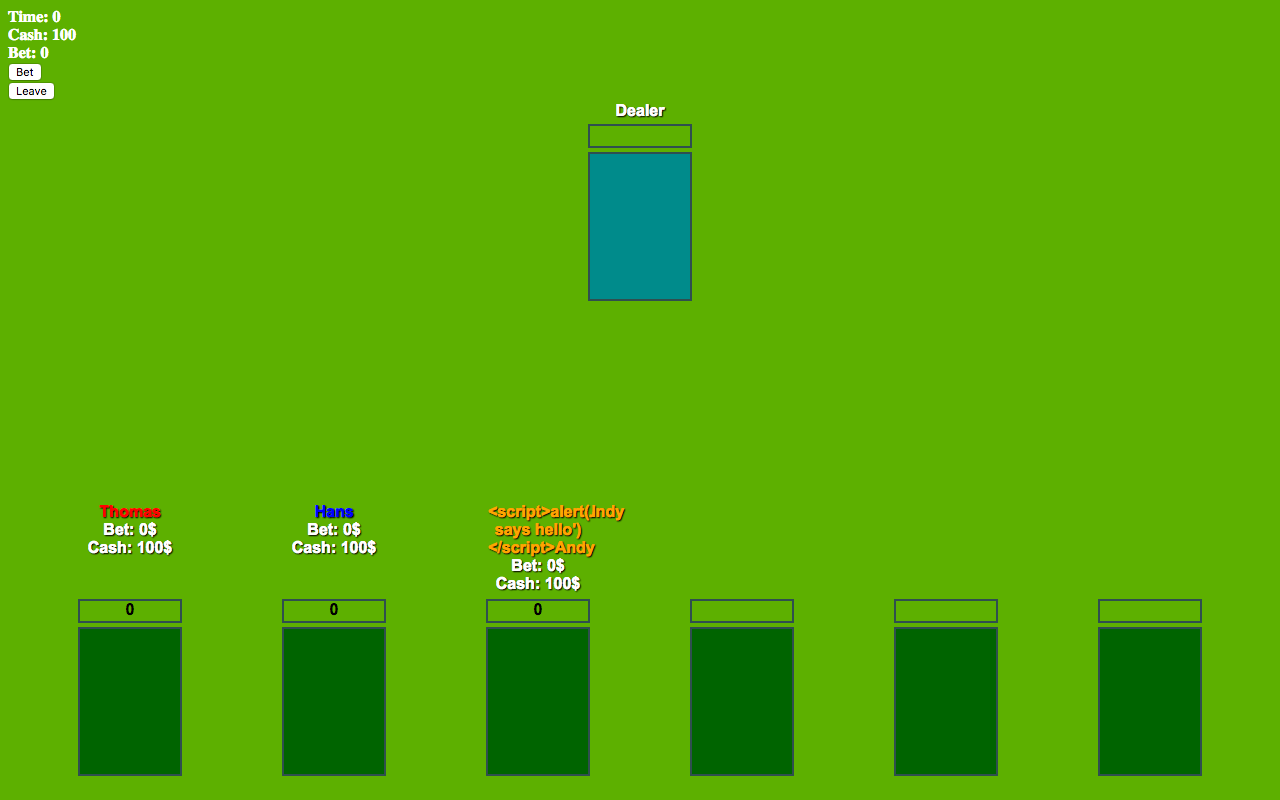
\includegraphics[width=0.65\textwidth]{images/xss_prevented}
  \caption{Image showing the failed xss injection}
  \label{img_xss_fail}
\end{figure}

Because the characters has been escaped properly, they show up as they should (see \autoref{img_xss_fail}). internally in the server the string is converted into this: \\\texttt{\&ltscript\&gtalert(\&\#x27Andy says hello\&\#x27)\&lt\&\#x2Fscript\&gtAndy} (this was copied from the console.)


% #=#=#=#=#=#=#=#=#=#=#=#=#=#=#=#=#=#=#=#=#=#=#=#=#=#=#=#=#=#=#=#=#=#=#=#=#=#=#=#=#


\section{Conclusion}
\textit{This section concludes the }

The Cross Site Scripting (xss) was successfully escaped, and has made it more inconvenient for attackers to inject JavaScript into the website.

\label{page_b4_appendices}


% #=#=#=#=#=#=#=#=#=#=#=#=#=#=#=#=#=#=#=#=#=#=#=#=#=#=#=#=#=#=#=#=#=#=#=#=#=#=#=#=#


\clearpage
\rfoot{ }
\addcontentsline{toc}{section}{References}	
\bibliographystyle{IEEEtran}
\bibliography{references.bib}

\listoffigures
\listoflistings


% #=#=#=#=#=#=#=#=#=#=#=#=#=#=#=#=#=#=#=#=#=#=#=#=#=#=#=#=#=#=#=#=#=#=#=#=#=#=#=#=#


\begin{appendices}
\section{How to Run}
\label{app_h2r}
To run the server, you need to have npm (it can be downloaded along with
  node here: \url{https://nodejs.org/en/download/}).

Run the following commands, in the server directory, to start the server:
\begin{minted}[firstnumber=1, bgcolor=white]{sh}
	$ npm install
\end{minted}
  
Install bower by running this command, in the command line to install
bower: (from: \url{https://bower.io})\\
NPM might need root permissions to install bower as it is installed globally (-g).

\begin{minted}[firstnumber=1, bgcolor=white]{sh}
	$ npm install -g bower
\end{minted}

To start the server, now you simply just has to run the following command.

\begin{minted}[firstnumber=1, bgcolor=white]{sh}
	$ npm start
\end{minted}

Now the server should be up and running.

To connect a client to the server, go to \url{http://localhost:13337/} (or click the link)
\end{appendices}

\end{document}